\PassOptionsToPackage{table}{xcolor}
\documentclass{SkripsiUnesa}
\loadglsentries{Istilah.tex}

\begin{document}

\Judul{Peramalan Harga Minyak Mentah Menggunakan \textit{Geometric Brownian Motion} Termodifikasi Kalman Filter}

\JudulEng{Forecasting Crude Oil Prices Using Geometric Brownian Motion Modified by Kalman Filter}

\Nama{Rafi Rachmad Ramadhan}

\NIM{20030214023}

\ProgramStudi{Sarjana Matematika}

\Programme{Bachelor of Mathematics}

\Tahun{2025}

\Fakultas{Matematika dan Ilmu Pengetahuan Alam}{MIPA}

\Faculty{Mathematics and Natural Sciences}

\Universitas{Universitas Negeri Surabaya}

\Institution{State University of Surabaya}

\KPS{Prof. Dr. Raden Sulaiman, M.Si.}

\NIPkps{196712031993021001}

\Dekan{Prof. Dr. Wasis, M.Si.}

\NIPDekan{196712031993021001}

\Pembimbing{Dimas Avian Maulana, S.Si., M.Si.}
           {}

\NIPPembimbing{199010072015041001}
              {}

\Penguji{A'yunin Sofro, M.Si., Ph.D.}
        {Affiati Oktaviarina, S.Si., M.Sc.}
        {}

\NIPPenguji{198008232005012002}
           {197810222006042001}
           {}

\Ahli{Dr. Rahmawati Erma Standsyah, M.Si.}

\NIPahli{198912112024062002}

\TanggalUji{12 Mei 2025} %Gunakan ini jika melakukan uji pakar

\TanggalDisetujui{25 Mei 2025}

\TanggalSidang{6 Juni 2025}


\Awal
\HalamanJudul
\SampulDalam

%Abstrak
\begin{Abstrak}
	
Perekonomian merupakan suatu bidang yang perlu mendapat perhatian di semua negara, baik negara maju maupun berkembang. Berbagai tantangan dan risiko masih membayangi perkembangan ekonomi global, terutama berasal dari inflasi yang terjadi di mayoritas negara-negara dunia. Pada proses perkembangan ekonomi, minyak mentah menjadi salah satu komoditas paling penting. Harga minyak mentah memiliki pengaruh yang signifikan terhadap perekonomian global. Hal ini dikarenakan kenaikan harga minyak akan meningkatkan biaya produksi, sehingga harga produk meningkat. Harga produk yang tinggi menyebabkan stagnansi pasar. Oleh karena itu, pemahaman berkelanjutan tentang pergerakan harga minyak mentah dunia penting untuk pengembangan dan pertumbuhan ekonomi. Salah satu model yang dapat digunakan dalam memprediksi pergerakan harga minyak ada lah \textit{Geometric Brown Motion} termodifikasi kalman filter. Dalam penelitian ini metode yang digunakan adalah \textit{Geometric Brown Motion} dan \textit{Geometric Brown Motion} termodifikasi kalman filter. Metode tersebut digunakan untuk memprediksi data harga minyak mentah per barel jenis \textit{West Texas Intermediate} dan \textit{brent}. Hasil dari penilitian ini menunjukkan bahwa metode \textit{Geometric Brown Motion} termodifikasi kalman filter	menghasilkan MAPE sebessar 1,108889\% untuk minyak mentah jenis West Texas Intermediate dan 1,097598\% untuk minyak mentah jenis \textit{brent}. MAPE tersebut lebih kecil dari lintasan terbaik \textit{Geometric Brown Motion} yang menghasilkan MAPE sebesar 2,562672\% untuk minyak mentah jenis West Texas Intermediate dan 2,537235\% untuk minyak mentah jenis \textit{brent}. Kedua metode tersebut menghasilkan MAPE $<$ 10\%	yang mengindikasikan bahwa kedua metode tersebut mempunyai tingkat akurasi peramalan yang tinggi untuk kasus ini.
	\katakunci{Minyak mentah, \textit{Geometric Brownian Motion}, Kalman Filter}
l\end{Abstrak}
\newpage

%Abstrak dalam Bahasa Inggris
\begin{Abstract}
	
Ebola is a deadly infectious disease, caused by the ebola virus from the family of Filoviridae, and genus Ebolavirus. Most of the transmission to humans is caused by animals or carcasses of infected animals, such as gorillas, monkeys, chimpanzees, bats and others. This virus can also be spread through sexual contact with the patient.
	
This study aims to reconstruct a mathematical model of the spreading of the Ebola virus with combinations of sexual and non-sexual transmission routes based on the SIR-SI epidemic model. The population within a community consists of the human population and the bat population. In the human population, it is divided into three cases, namely the vulnerable human population, the infected human population and the healed human population. Whereas, there are only two in the bat population that is the population of vulnerable bats and the population of infected bats. Infected humans can spread the virus to vulnerable humans through sexual intercourse.
\keywords{Stability analysis, Ebola virus, compartment diagram, the equilibrium point, linearization}
\end{Abstract}

\SuratPernyataan
%-------------------------------
\HalamanPersetujuan %digunakan untuk sidang skripsi
\HalamanPengesahan %digunakan untuk buku skripsi A5

\Prakata

Proses penciptaan karya ini merupakan kolaborasi tak kasat mata. Ada sumber-sumber yang menjadi pijakan, namun ide yang dihasilkan merupakan akumulasi dari berbagai perspektif yang bersinggungan. Ada berbagai sumber inspirasi yang tak terhitung dan karya ini adalah output dari sintesis tersebut. Oleh karena itu, terima kasih pada semua yang sudah membersamai penulis dalam penciptaan karya ini. karya ini disajikan dengan semangat apa adanya. Ia tak berpretensi menjadi sumber kebenaran tunggal, namun lebih sebagai jembatan untuk memicu pemikiran kritis. Terkadang, penemuan terbesar muncul dari interpretasi yang tak terduga.

\DaftarIsi
\DaftarTabel
\DaftarGambar
\DaftarSimbol
\renewcommand{\arraystretch}{1.2}
\begin{tabular}{p{0.1\textwidth} p{0.8\textwidth}}
	$m$ & Massa\\
	$p$ & Momentum\\
	$F$ & Gaya\\
	$\ax{\angln i}[\left(m\right)]$ & Nilai sekarang anuitas biasa (anuitas-\textit{immediate})\\
	$\ax**{\angln i}[\left(m\right)]$ & Nilai sekarang anuitas jatuh tempo (anuitas-\textit{due})\\
	$i^{(m)}$ & Tingkat bunga nominal tahunan yang dikapitalisasi $m$ kali dalam setahun\\
	$d^{(m)}$ & Tingkat diskonto nominal tahunan yang dikapitalisasi $m$ kali dalam setahun\\
	$v$ & Faktor diskonto (\textit{discount factor})\\
	$\amalg$ & Amalgamasi\\
	$\Re$ & Bagian real dari bilangan kompleks\\
	$\Im$ & Bagian imajiner dari bilangan kompleks 
\end{tabular}
\newpage

\Inti

\chapter{PENDAHULUAN}

\section{Latar Belakang}
Latar Belakang Masalah menjelaskan alasan-alasan rasional yang melandasi pentingnya penelitian tersebut dilakukan. Untuk membuat alasan rasional perlu diungkapkan kesenjangan antara kenyataan yang terjadi dibandingkan kenyataan yang diharapkan. Berbagai data, fakta, pendapat, keluhan dari lapangan/tempat penelitian perlu diungkap untuk memperkuat alasan perlunya dilakukan penelitian~\cite{Ver}

\section{Identifikasi Masalah}
Identifikasi Masalah menjelaskan kajian berbagai kemungkinan penyebab terjadinya masalah. Pada bagian ini perlu diungkap secara luas berbagai permasalahan yang mungkin untuk diteliti. Isi identifikasi masalah harus selaras dengan masalah yang diungkapkan pada latar belakang masalah.

\section{Batasan Masalah}
Batasan Masalah yakni penetapan masalah (dari berbagai masalah yang teridentifikasi) dengan mempertimbangkan berbagai aspek metodologis, kelayakan untuk diteliti, serta keterbatasan peneliti tanpa mengorbankan kebermaknaan arti, konsep, atau topik yang diteliti. Misalnya
\begin{daftar}
	\item Penelitian dilakukan dalam dalam bentuk simulasi numerik di komputer.
	\item Data kecepatan yang dipergunakan dalam penelitian ini diambil dari PT. Jasa Tirta I.
	\item Unsur-unsur hidrodinamika yang diteliti adalah kecepatan aliran.
	\item Pola penyebaran polutan yang diamati adalah arah panjang sungai (longitudinal) dan arah lebar sungai (lateral) selama tahun 2012.
	\item Parameter kualitas sungai yang digunakan adalah TSS (\textit{Total Suspended Solid}).
	\item Aliran sungai ditentukan bersifat kondisi Laminer.
	\item Kepadatan air sungai konstan karena air sungai adalah fluida yang tidak mampu mampat.
	\item Perubahan viskositas air cukup kecil sehingga dianggap konstan.
	\item Permukaan sungai adalah horizontal dan dinding sungai berkarakteristik relatif halus.
	\item Air sungai mengandung polutan TSS, dan polutan TSS menyebar mengikuti kecepatan aliran sungai.
	\item Pengaruh putaran bumi (gaya \textit{Coriolis}) sangat kecil sehingga dianggap nol.
	\item Gradien tekanan pada masing-masing sumbu ditentukan.
	\item Pengaruh angin sangat kecil sehingga gesekan di permukaan diasumsikan nol.
	\item Panjang sungai yang diukur dari pertemuan dua sungai adalah $1500m$ dan lebarnya $25m$
	\item Sungai yang menjadi objek penelitian ini adalah Kali Surabaya yang mengalir diantara Jalan Raya Mastrip (Karangpilang, Surabaya) dan Jalan Ngelom Rolak (Sepanjang, Sidoarjo)
\end{daftar}

\section{Rumusan Masalah}
Rumusan masalah berisi penegasan masalah yang akan diteliti sebagai hasil dari pembatasan masalah-masalah yang teridentifikasi. Rumusan masalah dituliskan dalam kalimat tanya. Misalnya:
\begin{daftar}
	\item Bagaimana model matematika penyebaran polutan pada pertemuan dua sungai.
	\item Bagaimana menerapkan Metode Volume Hingga skema \textit{QUICK} pada model penyebaran polutan pada pertemuan dua sungai tersebut.
	\item Bagaimana hasil penyebaran polutan di daerah aliran pertemuan dua sungai dengan Metode Volume Hingga skema \textit{QUICK}.
\end{daftar}

\section{Tujuan Penelitian}
Tujuan Penelitian menyatakan target yang akan dicapai melalui penelitian. Tujuan dirumuskan selaras/mengacu kepada rumusan masalah. Misalnya
\begin{daftar}
	\item Mengkaji dan menganalisis model matematika penyebaran polutan pada pertemuan dua sungai.	
	\item Menerapkan Metode Volume Hingga skema \textit{QUICK} dan menyelesaikan model matematika penyebaran polutan pada pertemuan dua sungai tersebut.
	\item Menyimulasikan dan memvisualisasikan penyelesaian numerik pola penyebaran polutan pada pertemuan dua sungai.
\end{daftar}

\section{Manfaat Penelitian}
Manfaat Penelitian menjelaskan manfaat hasil penelitian untuk kepentingan teoretis maupun praktis. Misalnya
\begin{daftar}
	\item Manfaat Teoretis 
	\item Manfaat Praktis
	\begin{daftar}
		\item Bagi Penulis
		\item Bagi Peneliti selanjutnya
		\item Bagi \textit{stakeholder} terkait (sebutkan \textit{stakeholder}nya)
	\end{daftar}
\end{daftar}

\section{Asumsi penelitian (jika ada)}
Asumsi penelitian (jika ada) adalah anggapan dasar tentang suatu hal yang dijadikan pijakan berpikir dan bertindak dalam melaksanakan penelitian. Asumsi dapat juga diartikan sebagai anggapan dasar yang menyebabkan suatu teori dapat berlaku. Asumsi dapat bersifat substantif atau metodologis. Asumsi substantif berkenaan dengan permasalahan penelitian, sedangkan asumsi metodologis berkenaan dengan metode penelitian.



\chapter{KAJIAN PUSTAKA}
Bab kajian pustaka bukan sekadar kumpulan kutipan, tetapi kutipan dan teori yang dibahas dan disintesis oleh peneliti/mahasiswa sehingga dapat memunculkan definisi, pemahaman baru, kerangka pikir, hipotesis dan/atau pertanyaan penelitian, serta mengembangkan instrumen yang sesuai dengan permasalahan yang diteliti. Secara umum, bab ini berisi landasan teori, kajian hasil penelitian yang relevan,

\section{Kajian Teori}
Kajian Teori menguraikan teori-teori terkait variabel penelitian meliputi definisi, konsep, asumsi, dan indikator yang digunakan untuk mengukur variabel tersebut dan sebagai landasan untuk mengembangkan instrumen penelitian. Kajian teori diperoleh dari literatur dan hasil penelitian yang relevan. Sumber rujukan untuk kajian teori dapat berupa buku teks, ensiklopedia, kamus, jurnal ilmiah, laporan penelitian, makalah seminar, prosiding, tesis ataupun disertasi. Artikel dalam internet juga dapat digunakan sebagai sumber rujukan apabila artikel ini dimuat dalam pusat-pusat kajian atau ditulis oleh penulis bereputasi. Namun, materi pembelajaran tidak dapat digunakan sebagai sumber rujukan karena belum mengalami uji publik melalui publikasi.

\subsection{Notasi Komutasi}
Jika simbol \( (m) \) ditambahkan ke sudut kanan atas, itu menunjukkan \textbf{nilai sekarang (Present Value, PV) dari suatu anuitas} di mana pembayaran dilakukan setiap \( \frac{1}{m} \) dari satu tahun selama \( n \) tahun, dan setiap pembayaran besarnya \( \frac{1}{m} \) dari satu unit.


\begin{align*}
	\ax{\angln i}[\left(m\right)] &= \frac{1 - v^n}{i^{(m)}}\\
	\ax**{\angln i}[\left(m\right)]  &= \frac{1 - v^n}{d^{(m)}}
\end{align*}


Di mana:
\begin{itemize}
	\item $\ax{\angln i}[\left(m\right)]$ menyatakan \textbf{nilai sekarang anuitas biasa} (anuitas-immediate), yaitu anuitas yang dibayar setiap \( \frac{1}{m} \) dari satu tahun pada akhir setiap periode.
	\item $\ax**{\angln i}[\left(m\right)]$ menyatakan \textbf{nilai sekarang anuitas jatuh tempo} (anuitas-due), yaitu anuitas yang dibayar di awal setiap periode.
	\item $i^{(m)}$ adalah \textbf{tingkat bunga nominal tahunan yang dikapitalisasi $m$ kali dalam setahun}.
	\item $d^{(m)}$ adalah \textbf{tingkat diskonto nominal tahunan yang dikapitalisasi $m$ kali dalam setahun}.
	\item $v = \frac{1}{1 + i}$ adalah faktor diskonto (discount factor), yang digunakan untuk menghitung nilai sekarang dari suatu pembayaran yang akan diterima di masa depan.
\end{itemize}

Dengan menggunakan rumus ini, kita dapat menghitung \textbf{nilai sekarang dari anuitas dengan pembayaran lebih sering} dari satu kali dalam setahun, seperti anuitas bulanan, kuartalan, atau semi-tahunan.


\begin{figure}[h!]
	\centering
	
\includegraphics[width=0.5\textwidth]{Gambar/logounesa}
	\caption{Logo Unesa}
	\label{fig:logounesa}
\end{figure}

\subsubsection{Rumus}
Rumus umum persamaan pythagoras diberikan oleh persamaan~\ref{eq:pythagoras} berikut ini
\begin{equation}
	a^2 + b^2 = c^2 \label{eq:pythagoras}
\end{equation}

Model penyebaran penyakit diberikan oleh sistem persamaan diferensial sebagai berikut:
\begin{align}
	\frac{dS}{dt} &= \beta S I\\
	\nonumber \frac{dI}{dt} &= -\beta S I
\end{align}

\begin{equation}
	\begin{aligned}
		\frac{dS}{dt} &= \beta S I\\
		\frac{dI}{dt} &= -\beta S I
	\end{aligned}
\end{equation}

\begin{equation}
	I = \int_0^{\infty} e^{at}~{dt}
\end{equation}

Matriks Identitas $3 \times 3$ diberikan oleh:
\begin{equation}
	I = \begin{bmatrix}
		1 & 0 & \cdots & 0\\
		0 & 1 & \cdots & \vdots\\
		\cdots & \cdots & \ddots &\vdots\\
		0 & 0 & \cdots & 1
	\end{bmatrix}
\end{equation}

\begin{theorem}[Teorema Keterbagian]
	Diberikan bilangan bulat  $a$, $b$, dan $c$ dengan $a \neq 0$ sehingga berlaku sifat-sifat berikut ini.
\end{theorem}

\begin{theorem}[Teorema Keterbagian]
	Diberikan bilangan bulat  $a$, $b$, dan $c$ dengan $a \neq 0$ sehingga berlaku sifat-sifat berikut ini.
\end{theorem}

\begin{proof}
	Berdasarkan $\cdots$
\end{proof}

\begin{definition}
	Diberikan bilangan bulat $a$ dan $b$ dengan $a \neq 0$. Jika $b$ merupakan kelipatan dari $a$, maka kita katakan bahwa  $a$ habis membagi $b$ atau dinotasikan $a|b$
\end{definition}

\begin{example}
	Diberikan bilangan bulat $a$ dan $b$ dengan $a \neq 0$. Jika $b$ merupakan kelipatan dari $a$, maka kita katakan bahwa  $a$ habis membagi $b$ atau dinotasikan $a|b$
\end{example}

\begin{theorem}
	Diberikan bilangan bulat  $a$, $b$, dan $c$ dengan $a \neq 0$ sehingga berlaku sifat-sifat berikut ini.
\end{theorem}

\section{Hasil Penelitian yang Relevan}
Hasil Penelitian yang relevan berfungsi memperkuat posisi penelitian yang dilakukan saat ini dengan melihat hasil-hasil penelitian yang sudah dilakukan. Hasil penelitian yang relevan juga digunakan sebagai dasar peneliti menyusun kerangka berpikir. Hasil penelitian yang relevan disajikan secara narasi dengan menganalisis hasil penelitian yang satu dengan hasil penelitian yang lain.

\section{Kerangka Berpikir}
Kerangka Berpikir berisikan gambaran logis dan rasional tentang bagaimana variable-variabel penelitian dapat saling berhubungan (korelasi). Kerangka berpikir akan mengarahkan peneliti kepada perumusan hipotesis. Penelitianyang tidak membuktikan hipotesis seperti penelitian dengan pendekatan kualitatif, tidak perlu menuliskan kerangka berpikir.

\section{Pertanyaan Penelitian dan/atau Hipotesis (jika ada)}
Pertanyaan penelitian merupakan penegasan dari rumusan masalah yang akan dicari jawabannya melalui penelitian. Hipotesis merupakan jawaban sementara terhadap rumusan masalah yang dinyatakan dengan kalimat pernyataan. Untuk penelitian yang tidak membuktikan hipotesis cukup menuliskan pertanyaan penelitian. Hipotesis atau pertanyaan penelitian harus selaras dan merupakan jabaran dari rumusan masalah.

\chapter{METODE PENELITIAN}
Bab ini akan menjelaskan metode penelitian yang digunakan dalam penelitian ini secara rinci. Metode penelitian ini mencakup jenis penelitian, tempat dan waktu penelitian, populasi dan sampel, definisi operasional variabel, teknik dan instrumen pengumpulan data, validitas dan reliabilitas instrumen, serta teknik analisis data.  Untuk memberikan gambaran visual mengenai alur penelitian secara keseluruhan, diagram alir penelitian disajikan sebagai berikut:
	\begin{figure}[h!]
		\centering
		\tikzstyle{startstop} = [rectangle, rounded corners=0.5cm, minimum width=2.5cm, minimum height=1cm, text centered, draw=black]
	\tikzstyle{io} = [trapezium, trapezium stretches=true, trapezium left angle=70,  trapezium right angle=110, minimum height=1cm, text centered, draw=black]
	\tikzstyle{process} = [rectangle, minimum width=2cm, minimum height=1cm, text centered, draw=black]
	\tikzstyle{decision} = [diamond, minimum height=1cm, aspect=2.5, text centered, draw=black]
	\tikzset{connector/.style={shape=signal, draw, signal to=south,text width=1cm,text height=0.5cm, align=center},
	}
	\tikzstyle{arrow} = [ultra thick,->,>=stealth]
	
	\begin{tikzpicture}[node distance=2cm]
		\node (start) [startstop] {Mulai};
		\node (in) [io, below of=start] {Data Saham};
		\node (pro2) [decision, below of=in] {Input Parameter};
		\node (pro3) [process, below of=pro2] {Hitung nilai $dt, u, d, p, v_{es}$ dan $S_{ij}$};
		\node (pro4) [process, below of=pro3] {Menghitung harga opsi saat jatuh tempo};
		\node (pro5) [process, below of=pro4] {Melakukan hitung mundur memperoleh $f_{0,0}$};
		\node (con) [connector, below of=pro5] {A};
		\node (stop) [startstop, below of=con] {Selesai};
		
		\draw [arrow] (start) -- (in);
		\draw [arrow] (in) -- (pro2);
		\draw [arrow] (pro2) -- (pro3);
		\draw [arrow] (pro3) -- (pro4);
		\draw [arrow] (pro4) -- (pro5);
		\draw [arrow] (pro5) -- (con);
		\draw [arrow] (con) -- (stop);		
	\end{tikzpicture}
	\caption{Alur penelitian}
	\end{figure}

\section{Jenis atau Desain Penelitian}
Peneliti perlu mengemukakan jenis atau desain penelitian sesuai dengan permasalahan yang akan diteliti.
\section{Tempat dan Waktu Penelitian}
Bagian ini berisi deskripsi mengenai kapan dan di mana penelitian akan dilakukan.
\section{Populasi dan Sampel Penelitian (jika ada)}
Populasi dan sampel digunakan bila wilayah sasaran peneliti cukup luas sehingga tidak memungkinkan semua anggota dijadikan responden sehingga peneliti melakukan penelitian dengan mengambil sampel secara representatif. Bila wilayah sasaran dapat dijangkau seluruhnya, subbab ini diberi nama sumber data atau subjek penelitian. Dalam bidang bahasa/sastra, digunakan istilah sumber data/subjek penelitian. Untuk penelitian yang menggunakan sampel perlu dijelaskan cara menentukan ukuran sampel dan teknik sampling yang digunakan.
\section{Definisi Operasional Variabel (jika ada)}
Definisi Operasional Variabel menjelaskan definisi masing-masing variabel disesuaikan dengan konteks penelitian. Definisi operasional dikembangkan dari teori, definisi konseptual, dan merupakan dasar bagi penentuan indikator- indikator dalam pengembangan instrumen penelitian.
\section{Teknik dan Instrumen Pengumpulan Data}
Pada bagian ini perlu dipaparkan teknik pengumpulan data yang digunakan dan instrumen yang dikembangkan. Peneliti perlu menjelaskan proses penyusunan instrumen dan pengujian kualitas instrumen.

\section{Validitas dan Reliabilitas Instrumen (jika ada)}
Instrumen dinyatakan layak sebagai alat pengumpul data bila memenuhi kriteria valid dan reliabel. Pada bagian ini perlu dijelaskan cara-cara penelusuran validitas dan reliabilitas instrumen. Untuk instrumen berupa tes kognitif dengan bentuk soal pilihan ganda, pengujian kualitas soal diuji dengan indeks kesulitan, daya beda, pengecoh, dan reliabilitas.
\section{Teknik Analisis Data}
Pada bagian ini perlu dijelaskan teknik analisis data yang digunakan termasuk uji persyaratan analisis yang dibutuhkan.
\section{Pelaksanaan Penelitian}
Kegiatan penelitian ini akan mengikuti jadwal yang telah disusun pada~\ref{tab:kegiatan} berikut.

\begin{table}[h!]
	\centering
	\caption{Pelaksanaan Penelitian}
	\label{tab:kegiatan}
	\begin{tabular}{|l|llll|llll|llll|llll|}
		\hline
		\multicolumn{1}{|c|}{}                           & \multicolumn{4}{c|}{I}                                                                                                                                                                        & \multicolumn{4}{c|}{II}                                                                                                                                                  & \multicolumn{4}{c|}{III}                                                                                                                                                 & \multicolumn{4}{c|}{IV}                                                                                                                                                  \\ \cline{2-17} 
		\multicolumn{1}{|c|}{\multirow{-2}{*}{Kegiatan}} & \multicolumn{1}{c|}{1}                        & \multicolumn{1}{c|}{2}                        & \multicolumn{1}{c|}{3}                        & \multicolumn{1}{c|}{4}                        & \multicolumn{1}{c|}{1}                        & \multicolumn{1}{c|}{2}                        & \multicolumn{1}{c|}{3}                        & \multicolumn{1}{c|}{4}   & \multicolumn{1}{c|}{1}                        & \multicolumn{1}{c|}{2}                        & \multicolumn{1}{c|}{3}                        & \multicolumn{1}{c|}{4}   & \multicolumn{1}{c|}{1}                        & \multicolumn{1}{c|}{2}                        & \multicolumn{1}{c|}{3}                        & \multicolumn{1}{c|}{4}   \\ \hline
		Studi Literatur                                  & \multicolumn{1}{c|}{\cellcolor[HTML]{9B9B9B}} & \multicolumn{1}{c|}{\cellcolor[HTML]{9B9B9B}} & \multicolumn{1}{c|}{}                         & \multicolumn{1}{c|}{}                         & \multicolumn{1}{c|}{}                         & \multicolumn{1}{c|}{}                         & \multicolumn{1}{c|}{}                         & \multicolumn{1}{c|}{}    & \multicolumn{1}{c|}{}                         & \multicolumn{1}{c|}{}                         & \multicolumn{1}{c|}{}                         & \multicolumn{1}{c|}{}    & \multicolumn{1}{c|}{}                         & \multicolumn{1}{c|}{}                         & \multicolumn{1}{c|}{}                         & \multicolumn{1}{c|}{}    \\ \hline
		Pengambilan Data                                 & \multicolumn{1}{c|}{}                         & \multicolumn{1}{c|}{}                         & \multicolumn{1}{c|}{\cellcolor[HTML]{9B9B9B}} & \multicolumn{1}{c|}{\cellcolor[HTML]{9B9B9B}} & \multicolumn{1}{c|}{\cellcolor[HTML]{9B9B9B}} & \multicolumn{1}{c|}{\cellcolor[HTML]{9B9B9B}} & \multicolumn{1}{c|}{}                         & \multicolumn{1}{c|}{}    & \multicolumn{1}{c|}{}                         & \multicolumn{1}{c|}{}                         & \multicolumn{1}{c|}{}                         & \multicolumn{1}{c|}{}    & \multicolumn{1}{c|}{}                         & \multicolumn{1}{c|}{}                         & \multicolumn{1}{c|}{}                         & \multicolumn{1}{c|}{}    \\ \hline
		Pengolahan Data                                  & \multicolumn{1}{l|}{}                         & \multicolumn{1}{l|}{}                         & \multicolumn{1}{l|}{}                         &                                               & \multicolumn{1}{l|}{}                         & \multicolumn{1}{l|}{\cellcolor[HTML]{9B9B9B}} & \multicolumn{1}{l|}{\cellcolor[HTML]{9B9B9B}} & \cellcolor[HTML]{9B9B9B} & \multicolumn{1}{l|}{\cellcolor[HTML]{9B9B9B}} & \multicolumn{1}{l|}{}                         & \multicolumn{1}{l|}{}                         &                          & \multicolumn{1}{l|}{}                         & \multicolumn{1}{l|}{}                         & \multicolumn{1}{l|}{}                         &                          \\ \hline
		Analisis Data                                    & \multicolumn{1}{l|}{}                         & \multicolumn{1}{l|}{}                         & \multicolumn{1}{l|}{}                         &                                               & \multicolumn{1}{l|}{}                         & \multicolumn{1}{l|}{}                         & \multicolumn{1}{l|}{}                         &                          & \multicolumn{1}{l|}{\cellcolor[HTML]{9B9B9B}} & \multicolumn{1}{l|}{\cellcolor[HTML]{9B9B9B}} & \multicolumn{1}{l|}{\cellcolor[HTML]{9B9B9B}} & \cellcolor[HTML]{9B9B9B} & \multicolumn{1}{l|}{}                         & \multicolumn{1}{l|}{}                         & \multicolumn{1}{l|}{}                         &                          \\ \hline
		Penarikan Kesimpulan                             & \multicolumn{1}{l|}{}                         & \multicolumn{1}{l|}{}                         & \multicolumn{1}{l|}{}                         &                                               & \multicolumn{1}{l|}{}                         & \multicolumn{1}{l|}{}                         & \multicolumn{1}{l|}{}                         &                          & \multicolumn{1}{l|}{}                         & \multicolumn{1}{l|}{}                         & \multicolumn{1}{l|}{}                         & \cellcolor[HTML]{9B9B9B} & \multicolumn{1}{l|}{\cellcolor[HTML]{9B9B9B}} & \multicolumn{1}{l|}{\cellcolor[HTML]{9B9B9B}} & \multicolumn{1}{l|}{}                         &                          \\ \hline
		Penulisan Skripsi                                & \multicolumn{1}{l|}{}                         & \multicolumn{1}{l|}{}                         & \multicolumn{1}{l|}{}                         &                                               & \multicolumn{1}{l|}{}                         & \multicolumn{1}{l|}{}                         & \multicolumn{1}{l|}{}                         & \cellcolor[HTML]{9B9B9B} & \multicolumn{1}{l|}{\cellcolor[HTML]{9B9B9B}} & \multicolumn{1}{l|}{\cellcolor[HTML]{9B9B9B}} & \multicolumn{1}{l|}{\cellcolor[HTML]{9B9B9B}} & \cellcolor[HTML]{9B9B9B} & \multicolumn{1}{l|}{\cellcolor[HTML]{9B9B9B}} & \multicolumn{1}{l|}{\cellcolor[HTML]{9B9B9B}} & \multicolumn{1}{l|}{\cellcolor[HTML]{9B9B9B}} & \cellcolor[HTML]{9B9B9B} \\ \hline
	\end{tabular}
\end{table}

\chapter{HASIL PENELITIAN DAN PEMBAHASAN}
Bab ini terdiri atas tiga bagian, yakni hasil penelitian, pembahasan, dan keterbatasan penelitian. Subbab pada bab 4 ini dapat disesuaikan dengan kebutuhan. Uraikan bab ini sesuai dengan alur berpikir dalam diagram alir

\section{Hasil Penelitian}
Hasil penelitian harus menjawab pertanyaan penelitian dan disusun menurut urutan pertanyaan penelitian/hipotesis.

\subsection{Pengelompokan Jenis Roti}
\begin{longtable}{|l|l|l|}
	\caption{Pengelompokan jenis roti di Lyly Bakery Lamongan} \\
	\hline
	No & Pengelompokan & Jenis Roti \\ \hline
	\multirow{10}{*}{1} & \multirow{10}{*}{Donat} & Donat strawberry marble \\ \cline{3-3}
	& & Donat chocolate peanut \\ \cline{3-3}
	& & Donat chocolate marble \\ \cline{3-3}
	& & Donat white choco almond \\ \cline{3-3}
	& & Donat icing sugar \\ \cline{3-3}
	& & Donat misis mix \\ \cline{3-3}
	& & Donat misis coklat \\ \cline{3-3}
	& & Donat chicken \\ \cline{3-3}
	& & Donat keju \\ \cline{3-3}
	& & Donat merah putih \\ \hline
	\multirow{7}{*}{2} & \multirow{7}{*}{Pastry Croissant} & Cum-cum contong mini \\ \cline{3-3}
	& & Cum cum sepatu \\ \cline{3-3}
	& & Croissant coklat marble \\ \cline{3-3}
	& & Croissant white almond \\ \cline{3-3}
	& & Grem kacang \\ \cline{3-3}
	& & Fruit danish \\ \cline{3-3}
	& & Apple danish \\ \hline
	\multirow{2}{*}{3} & \multirow{2}{*}{Puff pastry} & Molen coklat \\ \cline{3-3}
	& & Molen keju \\ \hline
	\multirow{6}{*}{4} & \multirow{6}{*}{Tawar} & Tawar kombinasi \\ \cline{3-3}
	& & Tawar kotak \\ \cline{3-3}
	& & Tawar kupas \\ \cline{3-3}
	& & Tawar kupas pandan \\ \cline{3-3}
	& & Tawar zebra \\ \cline{3-3}
	& & Tawar panjang roppang \\ \hline
	\multirow{2}{*}{5} & \multirow{2}{*}{Ban} & Ban hongkong \\ \cline{3-3}
	& & Ban hongkong pandan \\ \hline
	\multirow{8}{*}{6} & \multirow{8}{*}{Cupcake} & Cupcake fondan panda cewek \\ \cline{3-3}
	& & Cupcake fondan panda cowok \\ \cline{3-3}
	& & Cupcake white purple flower \\ \cline{3-3}
	& & Cupcake oreo choco cream \\ \cline{3-3}
	& & Cupcake cactus \\ \cline{3-3}
	& & Cupcake sesame street blue \\ \cline{3-3}
	& & Cupcake sesame street yellow \\ \cline{3-3}
	& & Cupcake kumbang \\ \hline
\end{longtable}

\subsection{Indeks Sensitivitas}
\begin{figure}[h!]
	\centering
	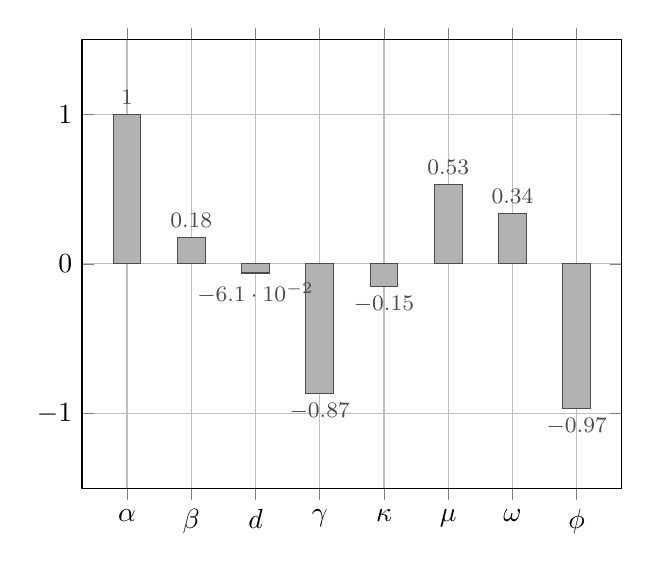
\begin{tikzpicture}
		\begin{axis}[
			ybar,
			ymin=-1.5,
			ymax=1.5,
			symbolic x coords={$\alpha$,$\beta$,$d$,$\gamma$,$\kappa$,$\mu$,$\omega$,$\phi$},
			xtick=data,
			nodes near coords,
			nodes near coords align={vertical},
			nodes near coords style={font=\footnotesize},
			grid=major,
			]
			\addplot[
			color=black!70,
			fill=black!30,
			] coordinates {
				($\alpha$,1)
				($\beta$,0.175)
				($d$,-0.061)
				($\gamma$,-0.87)
				($\kappa$, -0.15)
				($\mu$, 0.53)
				($\omega$, 0.34)
				($\phi$, -0.97)
			};
		\end{axis}
	\end{tikzpicture}
	\caption{Indeks sensitivitas}
\end{figure}

\subsection{Graf}
\begin{figure}[h!]
	\centering
	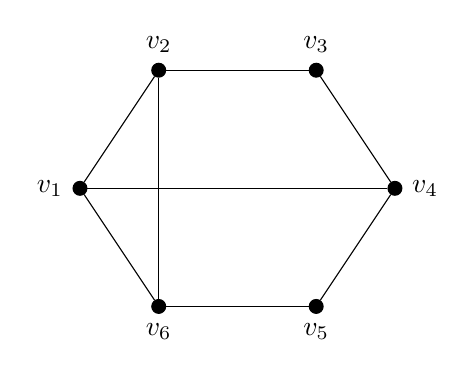
\begin{tikzpicture}[scale=1]
		% Nodes
		\node[circle, draw, fill=black, minimum size=5pt, inner sep=0pt, label=left:$v_1$] (v1) at (0,0) {};
		\node[circle, draw, fill=black, minimum size=5pt, inner sep=0pt, label=above:$v_2$] (v2) at (1,1.5) {};
		\node[circle, draw, fill=black, minimum size=5pt, inner sep=0pt, label=above:$v_3$] (v3) at (3,1.5) {};
		\node[circle, draw, fill=black, minimum size=5pt, inner sep=0pt, label=right:$v_4$] (v4) at (4,0) {};
		\node[circle, draw, fill=black, minimum size=5pt, inner sep=0pt, label=below:$v_5$] (v5) at (3,-1.5) {};
		\node[circle, draw, fill=black, minimum size=5pt, inner sep=0pt, label=below:$v_6$] (v6) at (1,-1.5) {};
		
		% Edges
		\draw (v1) -- (v2);
		\draw (v1) -- (v6);
		\draw (v1) -- (v4);
		\draw (v2) -- (v3);
		\draw (v3) -- (v4);
		\draw (v4) -- (v5);
		\draw (v5) -- (v6);
		\draw (v6) -- (v2);
		\draw (v6) -- (v5);
		\draw (v2) -- (v3);
	\end{tikzpicture}
	\caption{Graf $G$}
\end{figure}

\begin{figure}[h!]
	\centering
	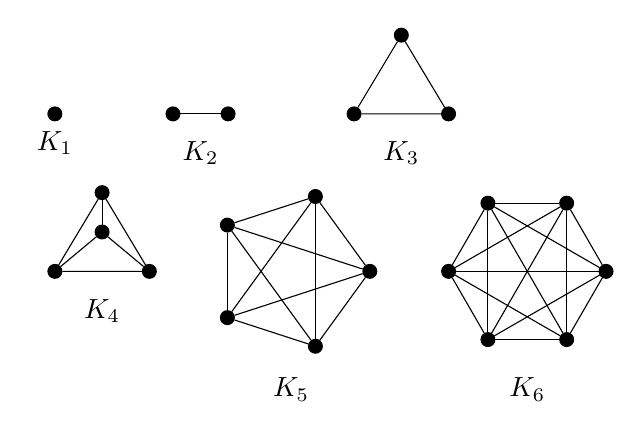
\begin{tikzpicture}[scale=1]
		
		% Row 1: K1, K2, K3
		% K1
		\node[circle, draw, fill=black, minimum size=5pt, inner sep=0pt, label=below:$K_1$] (k1) at (0,1) {};
		
		% K2
		\node[circle, draw, fill=black, minimum size=5pt, inner sep=0pt] (k21) at (1.5,1) {};
		\node[circle, draw, fill=black, minimum size=5pt, inner sep=0pt] (k22) at (2.2,1) {};
		\draw (k21) -- (k22);
		\node at (1.85,0.5) {$K_2$};
		
		% K3 (Triangle)
		\node[circle, draw, fill=black, minimum size=5pt, inner sep=0pt] (k31) at (3.8,1) {};
		\node[circle, draw, fill=black, minimum size=5pt, inner sep=0pt] (k32) at (5,1) {};
		\node[circle, draw, fill=black, minimum size=5pt, inner sep=0pt] (k33) at (4.4,2) {};
		\draw (k31) -- (k32) -- (k33) -- (k31);
		\node at (4.4,0.5) {$K_3$};
		
		% Row 2: K4, K5, K6
		% K4 (Tetrahedron)
		\node[circle, draw, fill=black, minimum size=5pt, inner sep=0pt] (k41) at (0,-1) {};
		\node[circle, draw, fill=black, minimum size=5pt, inner sep=0pt] (k42) at (1.2,-1) {};
		\node[circle, draw, fill=black, minimum size=5pt, inner sep=0pt] (k43) at (0.6,0) {};
		\node[circle, draw, fill=black, minimum size=5pt, inner sep=0pt] (k44) at (0.6,-0.5) {};
		\draw (k41) -- (k42) -- (k43) -- (k41);
		\draw (k41) -- (k44) -- (k42);
		\draw (k43) -- (k44);
		\node at (0.6,-1.5) {$K_4$};
		
		% K5 (Pentagon)
		\foreach \i in {0,72,144,216,288} {
			\node[circle, draw, fill=black, minimum size=5pt, inner sep=0pt] (k5\i) at ({3 + cos(\i)}, {-1 + sin(\i)}) {};
		}
		\foreach \i in {0,72,144,216,288} {
			\foreach \j in {0,72,144,216,288} {
				\ifnum\i<\j
				\draw (k5\i) -- (k5\j);
				\fi
			}
		}
		\node at (3,-2.5) {$K_5$};
		
		% K6 (Hexagon)
		\foreach \i in {0,60,120,180,240,300} {
			\node[circle, draw, fill=black, minimum size=5pt, inner sep=0pt] (k6\i) at ({6 + cos(\i)}, {-1 + sin(\i)}) {};
		}
		\foreach \i in {0,60,120,180,240,300} {
			\foreach \j in {0,60,120,180,240,300} {
				\ifnum\i<\j
				\draw (k6\i) -- (k6\j);
				\fi
			}
		}
		\node at (6,-2.5) {$K_6$};
		
	\end{tikzpicture}
	\caption{Graf Komplit}
\end{figure}

\begin{figure}[h!]
	\centering
	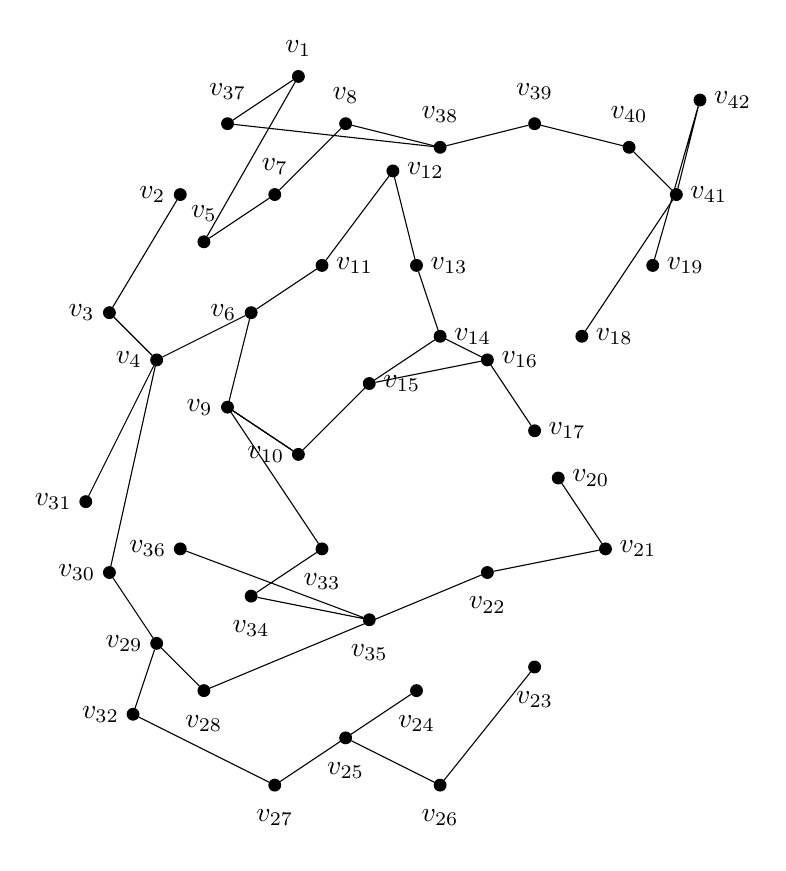
\begin{tikzpicture}[scale=3, every node/.style={circle, draw, fill=black, inner sep=1.5pt}]
		% Penempatan simpul berdasarkan estimasi dari gambar
		\node (v1) at (0,2) [label=above:$v_1$] {};
		\node (v2) at (-0.5,1.5) [label=left:$v_2$] {};
		\node (v3) at (-0.8,1) [label=left:$v_3$] {};
		\node (v4) at (-0.6,0.8) [label=left:$v_4$] {};
		\node (v5) at (-0.4,1.3) [label=above:$v_5$] {};
		\node (v6) at (-0.2,1) [label=left:$v_6$] {};
		\node (v7) at (-0.1,1.5) [label=above:$v_7$] {};
		\node (v8) at (0.2,1.8) [label=above:$v_8$] {};
		\node (v9) at (-0.3,0.6) [label=left:$v_9$] {};
		\node (v10) at (0,0.4) [label=left:$v_{10}$] {};
		\node (v11) at (0.1,1.2) [label=right:$v_{11}$] {};
		\node (v12) at (0.4,1.6) [label=right:$v_{12}$] {};
		\node (v13) at (0.5,1.2) [label=right:$v_{13}$] {};
		\node (v14) at (0.6,0.9) [label=right:$v_{14}$] {};
		\node (v15) at (0.3,0.7) [label=right:$v_{15}$] {};
		\node (v16) at (0.8,0.8) [label=right:$v_{16}$] {};
		\node (v17) at (1,0.5) [label=right:$v_{17}$] {};
		\node (v18) at (1.2,0.9) [label=right:$v_{18}$] {};
		\node (v19) at (1.5,1.2) [label=right:$v_{19}$] {};
		\node (v20) at (1.1,0.3) [label=right:$v_{20}$] {};
		\node (v21) at (1.3,0) [label=right:$v_{21}$] {};
		\node (v22) at (0.8,-0.1) [label=below:$v_{22}$] {};
		\node (v23) at (1,-0.5) [label=below:$v_{23}$] {};
		\node (v24) at (0.5,-0.6) [label=below:$v_{24}$] {};
		\node (v25) at (0.2,-0.8) [label=below:$v_{25}$] {};
		\node (v26) at (0.6,-1) [label=below:$v_{26}$] {};
		\node (v27) at (-0.1,-1) [label=below:$v_{27}$] {};
		\node (v28) at (-0.4,-0.6) [label=below:$v_{28}$] {};
		\node (v29) at (-0.6,-0.4) [label=left:$v_{29}$] {};
		\node (v30) at (-0.8,-0.1) [label=left:$v_{30}$] {};
		\node (v31) at (-0.9,0.2) [label=left:$v_{31}$] {};
		\node (v32) at (-0.7,-0.7) [label=left:$v_{32}$] {};
		\node (v33) at (0.1,0) [label=below:$v_{33}$] {};
		\node (v34) at (-0.2,-0.2) [label=below:$v_{34}$] {};
		\node (v35) at (0.3,-0.3) [label=below:$v_{35}$] {};
		\node (v36) at (-0.5,0) [label=left:$v_{36}$] {};
		\node (v37) at (-0.3,1.8) [label=above:$v_{37}$] {};
		\node (v38) at (0.6,1.7) [label=above:$v_{38}$] {};
		\node (v39) at (1,1.8) [label=above:$v_{39}$] {};
		\node (v40) at (1.4,1.7) [label=above:$v_{40}$] {};
		\node (v41) at (1.6,1.5) [label=right:$v_{41}$] {};
		\node (v42) at (1.7,1.9) [label=right:$v_{42}$] {};
		
		% Koneksi antar simpul sesuai gambar
		\draw (v1) -- (v37) -- (v38) -- (v39) -- (v40) -- (v41) -- (v42) -- (v19);
		\draw (v1) -- (v5) -- (v7) -- (v8) -- (v38);
		\draw (v2) -- (v3) -- (v4) -- (v6) -- (v9) -- (v10);
		\draw (v6) -- (v11) -- (v12) -- (v13) -- (v14) -- (v16) -- (v17);
		\draw (v9) -- (v33) -- (v34) -- (v35) -- (v36);
		\draw (v31) -- (v4) -- (v30) -- (v29) -- (v28);
		\draw (v29) -- (v32) -- (v27) -- (v24) -- (v25) -- (v26) -- (v23);
		\draw (v20) -- (v21) -- (v22);
		\draw (v18) -- (v41);
		\draw (v22) -- (v28);
		\draw (v14) -- (v15);
		\draw (v9) -- (v10) -- (v15) -- (v16);
		
	\end{tikzpicture}
	\caption{Graf Dual}
	\label{fig:Dual}
\end{figure}
Berdasarkan~\ref{fig:Dual}, graf tersebut dapat direpresentasikan dalam titik dan sisi sebagai berikut:
\begin{align*}
	G &= (V(G), E(G))\\
	V &= \left\lbrace 
	\begin{array}{llllllll}
		v_1, & v_2, & v_3, & v_4, & v_5, & v_6, & v_7, & v_8,\\
		v_9, & v_{10}, & v_{11}, & v_{12}, & v_{13}, & v_{14}, & v_{15}, & v_{16},\\
		v_{17}, & v_{18}, & v_{19}, & v_{20}, & v_{21}, & v_{22}, & v_{23}, & v_{24},\\
		v_{25}, & v_{26}, & v_{27}, & v_{28}, & v_{29}, & v_{30}, & v_{31}, & v_{32},\\
		v_{33}, & v_{34}, & v_{35}, & v_{36}, & v_{37}, & v_{38}, & v_{39}, & v_{40},\\
		v_{41}, & v_{42}
	\end{array}
	\right\rbrace
\end{align*}

\begin{align*}
	E &= \left\lbrace 
	\begin{array}{llllllll}
		(v_1v_2), & (v_1v_{37}), & (v_2v_3), & (v_2v_4), & (v_2v_5), & (v_2v_{37}), & (v_3v_4), & (v_3v_{30}),\\
		(v_4v_5), & (v_4v_6), & (v_4v_{30}), & (v_4v_{31}), & (v_5v_6), & (v_5v_7), & (v_5v_{11}), & (v_5v_{37}),\\
		(v_6v_9), & (v_6v_{11}), & (v_6v_{31}), & (v_7v_8), & (v_7v_{11}), & (v_7v_{37}), & (v_8v_{11}), & (v_8v_{12}),\\
		(v_8v_{38}), & (v_9v_{10}), & (v_9v_{11}), & (v_9v_{31}), & (v_9v_{32}), & (v_9v_{33}), & (v_{10}v_{11}), & (v_{10}v_{15}),\\
		(v_{10}v_{17}), & (v_{10}v_{33}), & (v_{10}v_{35}), & (v_{11}v_{12}), & (v_{11}v_{15}), & (v_{12}v_{13}), & (v_{12}v_{15}), & (v_{12}v_{38}),\\
		(v_{13}v_{14}), & (v_{13}v_{15}), & (v_{13}v_{16}), & (v_{13}v_{38}), & (v_{13}v_{39}), & (v_{13}v_{41}), & (v_{14}v_{15}), & (v_{14}v_{16}),\\
		(v_{14}v_{17}), & (v_{14}v_{18}), & (v_{15}v_{16}), & (v_{15}v_{17}), & (v_{17}v_{18}), & (v_{17}v_{20}), & (v_{17}v_{35}), & (v_{18}v_{19}),\\
		(v_{18}v_{20}), & (v_{18}v_{21}), & (v_{18}v_{41}), & (v_{19}v_{21}), & (v_{19}v_{41}), & (v_{19}v_{42}), & (v_{20}v_{21}), & (v_{20}v_{22}),\\
		(v_{20}v_{23}), & (v_{20}v_{35}), & (v_{21}v_{23}), & (v_{22}v_{23}), & (v_{22}v_{24}), & (v_{22}v_{25}), & (v_{22}v_{26}), & (v_{22}v_{28}),\\
		(v_{22}v_{36}), & (v_{23}v_{26}), & (v_{24}v_{25}), & (v_{24}v_{27}), & (v_{25}v_{26}), & (v_{27}v_{28}), & (v_{27}v_{29}), & (v_{28}v_{29}),\\
		(v_{28}v_{30}), & (v_{28}v_{36}), & (v_{29}v_{31}), & (v_{29}v_{32}), & (v_{29}v_{34}), & (v_{30}v_{31}), & (v_{31}v_{32}), & (v_{32}v_{33}),\\
		(v_{32}v_{34}), & (v_{33}v_{34}), & (v_{33}v_{35}), & (v_{34}v_{36}), & (v_{35}v_{36}), & (v_{37}v_{38}), & (v_{38}v_{39}), & (v_{39}v_{40}),\\
		(v_{39}v_{41}), & (v_{40}v_{41}), & (v_{40}v_{42}), & (v_{41}v_{42})
	\end{array}
	\right\rbrace
\end{align*}

\begin{align*}
	E &= \left\lbrace e_1, e_2, \dots, e_{100} \right\rbrace\\
	R &= \left\lbrace r_1, r_2, \dots, r_{60} \right\rbrace
\end{align*}

\section{Pembahasan}
Bagian pembahasan merupakan bagian penting dari penelitian dan letaknya terpisah dari subbab hasil penelitian. Bagian pembahasan memuat telaah kritis terhadap penelitian menggunakan perspektif dari berbagai teori yang relevan yang telah dibahas pada Bab II.

\section{Keterbatasan Penelitian}
Keterbatasan penelitian merupakan keterbatasan terkait metodologi bukan keterbatasan terkait waktu, biaya, atau logistik penelitian. Keterbatasan penelitian juga tidak terkait jumlah sampel atau variabel penelitian karena hal ini telah ditentukan sebelumnya.

\chapter{SIMPULAN DAN SARAN}
Bab ini memuat tiga subbab yaitu simpulan, implikasi, dan saran.

\section{Simpulan}
Simpulan harus pendek, merupakan deskripsi esensial, cenderung berbentuk pernyataan kualitatif, dan bukan angka-angka. Simpulan merupakan rangkuman dari jawaban pertanyaan penelitian atau hasil uji hipotesis dan sekaligus merupakan pemecahan permasalahan yang ada pada rumusan masalah

\section{Implikasi}
Implikasi adalah konsekuensi lebih lanjut dari temuan dalam simpulan. Biasanya implikasi menggunakan bahasa saran tetapi belum operasional.

\section{Saran}
Saran merupakan rekomendasi yang ditujukan kepada berbagai pihak terkait hasil penelitian dan menggunakan bahasa yang operasional. Implikasi dan saran harus sesuai dengan hasil penelitian yang telah terangkum dalam simpulan.

\nocite{*}

\DaftarPustaka{Pustaka}
\Glosarium
\BukaLampiran

\lampiran{Surat Keterangan Uji Ahli} %gunakan ini jika memerlukan keterangan uji ahli, misal kuesioner
\UjiAhli

\lampiran{\textit{Source code}}
\lstinputlisting[language=python]{epidemiology.py}

\lampiran{Biodata Penulis}
\biodata{Gambar/foto}
Ryan took part in the BBC series Strictly Come Dancing. He was partnered with professional dancer Nadiya Bychkova and was the second contestant to be eliminated on 7 October 2018. In 2019, Ryan starred in Celebs Go Dating on E4 and released his first single after nine years called "Ghost". Ryan subsequently released two further solo singles in 2020, "Mockingbirds" and Swayed".

Ryan reunited with Blue in 2011 and in 2022 they released singles "Haven't Found You Yet" and "Dance with Me" from their sixth studio album Heart \& Soul.

\end{document}
